\section{Attacks on Hardware}
\label{sec:curr_attacks}
After getting more familiar with the attack target and its architecture, an occasionally complicated process \citep{sergei:thesis} \citep{hwre},  one is made aware of the protective mechanisms of their target and, depending on the sophistication of the protections and the goals of the attacker, one should decide between \emph{passively} or \emph{actively} attacking the chip. When performing a passive attacks one monitors the chip's normal operation and tries to infer the input-output mapping whereas in active attacks the attacker manipulates the chip or its operating environment with the aim of obtaining insight on the chips inner workings by abusing abnormal behaviour. Attacks on MCUs may attempt to recover cryptographic keys or the firmware on the device and do not necessarily target the hardware itself but can exploit flaws in algorithmic design and implementation and protocol failures, inter-component communication patterns \citep{anderson:cautionary_note} \citep{kocher:DPA} or exploiting memory remanence \citep{sergei:thesis} \citep{gutman:memory_remanence}.

The following discussion closely follows Skorobogatov \citep{sergei:thesis} and the Hardware Reverse Engineering course material \citep{hwre}.

	\subsection{Non-Invasive Attacks}
	Non-invasive attacks are attacks which require no depackaging or special preparation of the chip and hence leave little tamper evidence behind. These attacks might be very time consuming to find and are not guaranteed to be successful (researchers report an average exloitation rate of \~50\% \citep{sergei:thesis} \citep{glitches_paper}), but are very cheap to replicate once found.
	
	\red{get more technical on DPA}
A popular non-invasive technique is power analysis, exploiting the fact that different instructions executing on a CPU require different amounts of power \citep{website:riscure} \citep{kocher:DPA} and hence one can infer which instruction is executing on a CPU by analysing a power trace generated by the MCU. These attacks are easy and relatively inexpensive to perform as they only require inserting a resistor in series with the MCU's power or ground, for avoiding noise \citep{sergei:thesis}, input and then equipment for sampling voltage differences for constricting a trace \citep{kocher:DPA}. 

Simple Power Analysis(SPA) involves direct observation of the MCU when it performs cryptographic operations and can leak information about both the keys and the cryptographic operations themselves like the nature or structure of the algorithm \citep{kocher:DPA} \citep{anderson:tamper_resistance}. Differential Power Analysis(DPA) extracts sensitive information by using statistical techniques on very large traces. The techniques involves obtaining power traces of known cipher-texts (but not necessarily knowing the corresponding plain-texts) and individual bits of the key are recovered by analysing the statistical differences in power consumption \citep{kocher:DPA} \citep{anderson:tamper_resistance}.

	\begin{figure}
		\center
		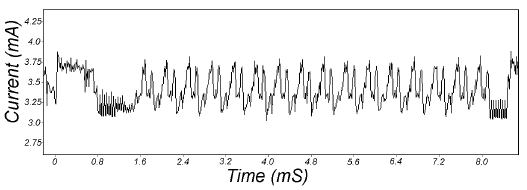
\includegraphics[scale=0.6]{img/power_des.png}
		\caption{\footnotesize Power trace during a DES encryption, where the 16 rounds are clearly visible.(reproduced from: \protect\citep{kocher:DPA}).}
		\label{fig:des_power}		
	\end{figure}

	
	Another popular attack type is inducing glitches or faults, which can be injected in a MCU by making it operate outside its operating temperatures, voltage or clock frequency and exploiting the resulting undefined behaviour of the MCU \citep{sergei:thesis} \citep{avr_mega}. Although inducing a fault is easy, inducing an exploitable fault is hard, but can be achieved by systematic search \citep{sergei:thesis} \citep{glitches_paper} \citep{website:riscure}. \emph{Power glitches} and \emph{clock glitches} aim to make the CPU skip or execute incorrect instructions by applying transients. This attack is board-specific and can target in individual components of an MCU and a systematic search can deduce which components are affected by a given glitch sequence. Clock glitches involve increasing the clock signal frequency so that some flip flops sample their input before being updated and hence report an incorrect value \citep{sergei:thesis} and are mainly aimed against software-based protection mechanisms, affecting CPU operation by supplying the CPU with incorrect data (or instructions). Power glitches work by supplying either too much power or too little, shifting transistors' threshold and causing flip-flops to read their state incorrectly and as a result need to be carefully synchronised with the internal clock and prolonged attacks might damage the board \citep{sergei:thesis}. Glitch attacks are especially dangerous as they may abuse the program counter in order to map out the memory \citep{glitches_paper} \citep{anderson:cautionary_note} \citep{sergei:thesis}.

	\begin{figure}
		\center
		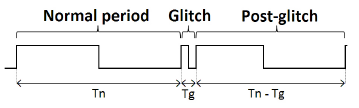
\includegraphics[scale=0.7]{img/clock_glitch.png}
		\caption{\footnotesize Illustration of the principle of a clock-glitch attack.(reproduced from: \protect\citep{glitches_paper}).}
		\label{fig:glitch}		
	\end{figure}

	Data remanence in SRAM cells is another possible attack vector, as prolonged exposure of SRAM cells to the same values can make the cells 'remember' their state. Hot-carrier effects and electromigration effects can cause physical alteration to a cell's surface, leaving an excess charge which can alter a cell's threshold voltage noticeably and reveal which type of signal was most common for particular cell ( 0 or 1) \citep{gutman:memory_remanence}. Furthermore, because of the hit-carrier effect high speed electrons can be trapped in the gate oxide to remain there as excess charge. Cooling the memory down can prolong the time for this charge to deplete, thus prolonging the time available for data recoverability  \citep{gutman:memory_remanence} \citep{sergei:RAM} \citep{sergei:thesis}. Hot-carrier effects also apply to EEPROM memory, but to a lesser extent, as material-wise one can only tell virgin-cells from used cells and there might be a shift in the threshold voltages of erased cells\citep{gutman:memory_remanence} \citep{sergei:thesis}. 
	
	
	Finally, due to its simplicity, another common attack includes timing attacks, which in MCUs is even more noticable as instructions have fixed execution cycles. Timing attacks exploit the software implementation of cryptographic algorithms. Compiler optimisations and other implementation choices might make the execution time of an algorithm dependent on the input and the secret key rather being fixed for any input, for example when input is compared byte-wise with a key and rejected when the first non-matching byte is found, rather than first consuming the whole input string. Furthermore different instructions have different execution times (\texttt{RET} is considerably slower than \texttt{INC r1} \citep{atmega_manual}) and thus one could collect timing information for various input messages and systematically brute-force the key. If timing information is correlated with power analysis then defences such as constant instruction execution time could be defeated. One might use \texttt{NOP}s in the case of a wrong key in order for rejection and confirmation responses to have constant execution time but \texttt{NOP} consumes substantially less power than \texttt{LD} \citep{glitches_paper} and correlating timing and power consumption information would reveal this.

	\subsection{Semi-Invasive Attacks and Invassive attacks}
	Attacks under this category require depackaging of the chip and, while semi-invasive attacks do not require complicated machinery or any sort of contact with the die surface, invasive attacks require physical contact and partial depassivation and are therefore a lot more expensive, time consuming, complicated and leave tamper-evidence \citep{sergei:thesis} \citep{gutman:memory_remanence}. Decapsulation of the chip can happen in a number of ways, depending on the packaging \citep{hwre} \citep{ic_decap}. HNO$_3$ or H$_2$SO$_4$ could be used if the packging is made out of epoxy resin and, if one wants to remove the residue or dirt left from chemical etcing, then bathe the die in an ultrasonic bath with acetone or distiled water \citep{sergei:thesis} \citep{hwre} \citep{ic_decap}. Alternatively, one could send the chip to a hardware analysis lab and get them to open the chip \citep{website:hacking_the_pic}. 
	
	Once the die surface is exposed it could be attacked with UV light. Older chips and chips that are designed to withstand low-cost non-invasive attacks are susceptible to having parts of the memory altered if it is exposed under UV light \citep{sergei:thesis} \citep{hwre}, altering memory contents or resetting security fuses that prevent read-back of the memory by sufficient exposure under UV light. Mechanisms that rely on fuses or checking a memory address for a particular value are susceptible to this kind of attack.

	A possible step after decapsulation is reverse-engineering the MCU in order to understand how it does its task, potentially having to image numerous layers. Low cost devices can usually be imaged from the top side, since they do not contain many layers or overlapping layers. If layers are overlapping mechanical etching could be used to take successive layers off \citep{ic_decap} \citep{hwre} or one could image the chip from the rear \citep{hwre} \citep{sergei:thesis}. Backside imaging involves shining IR light on the rear side of the chip and imaging it from this angle, since it is a mirror-image of the front side. This is possible because, usually, light shown through the backside does not have to go though multiple layers and hence protective metal meshes or normal chip layers are avoided \citep{hwre}. On some chips it is possible to extract ROM contents via this technique by directly observing the memory \citep{sergei:thesis}. An alternative to IR light would be the use of lasers and the photoelectric effect for imaging, and Optical Beam Induced Current and Light Induced Voltage Alteration are the two most common techniques for failure analysis that take advantage of the photoelectric effect. These techniques involve shining lasers on the semiconductor surface in order to alter some property; in OBIC a slight current is created and by analysing this one can deduce the device's properties (including defects and anomalies) and produce an image of the the board being scanned, while in LIVA the board is connected to constant power supply and changes in the power supply are monitored as laser is shone on the device, allowing one to deduce the device's characteristics and construct an image \citep{cole:OBIC}. Lasers can also be used to read the state of memory cells in CMOS SRAM \citep{sergei:thesis} or in order to corrupt memory contents by localized heating, by shooting a laser on a memory cell long enough for its state to change \citep{website:riscure} \citep{sergei:thesis}.
	
	For speeding up reverse engineering of a chip, one might physically need to modify it. This is certainly the case for invasive attacks \citep{sergei:thesis} \citep{gutman:memory_remanence}. Specialized equipment is hard and expensive to find, but one could go for slightly older second-hand equipment with a basic setup including a microscope (optical is good but SEM is better \citep{sergei:thesis} \citep{hwre}), a moving base for the chip to go onto, micro-positioners and probing needles with $\mu$m-thick precision and the test circuitry and hardware used, all of which could be obtained for under \$5000 \citep{low_cost_probing} \citep{gutman:memory_remanence} \citep{sergei:thesis} \citep{hwre}. Furthermore one could use cuting lasers in order to etch through the passivation layer in order to accurately position their probes \citep{sergei:thesis}, as well as destroy circuitry. A more reliable method includes using focused ion beams for accessing deeper chip layers for creating and destroying interconnects, but it is extremely expensive to obtain the machinery and knowledge on how to use it is essential (although renting time on one is an option) \citep{sergei:thesis} \citep{hwre} \citep{gutman:memory_remanence}. 